\setlength{\parskip}{10pt}
\setlength{\parindent}{0pt}
\chapter{Introduzione}
\label{chap:intro}

Uno dei problemi che da sempre affliggono gli appassionati di videogiochi, soprattutto chi lo fa in ambito competitivo, è la latenza totale del sistema, ossia l'intervallo di tempo che passa tra un'azione nel mondo fisico, come la pressione di un tasto del mouse, e la visualizzazione del risultato sullo schermo.\\
Il problema non è nulla di nuovo, ed esiste dagli albori della computer grafica in tempo reale. Nel 2012, John Carmack, uno dei più influenti e famosi sviluppatori di engine per videogiochi, ha puntualizzato questo problema nel seguente \textit{tweet}\footnote{\url{https://twitter.com/id_aa_carmack/status/193480622533120001}}:
\begin{quotation}
	``I can send an IP packet to Europe faster than I can send a pixel to the screen.  How f’d up is that?''
\end{quotation}
Dal 2012 ad oggi molte cose sono cambiate: da una parte la diffusione di tecnologie come display ad alto \textit{refresh rate}, VESA Adaptive Sync (e la controparte proprietaria Nvidia G-Sync), e le ottimizzazioni nei driver per applicazioni a latenza critica hanno migliorato la situazione, ma dall'altra l'aumento vertiginoso della complessità delle pipeline grafiche dei videogiochi, l'utilizzo di tecniche di \textit{antialiasing} temporale, il \textit{checkerboard rendering}, il \textit{triplo buffering}, lo \textit{smoothing} del movimento del mouse, e il \textit{compositing} del desktop hanno peggiorato notevolmente la situazione, al punto che molti considerano qualsiasi \textit{framerate} sotto i 60 FPS ingiocabile per via del ritardo di input percepibile.

Si può intuire fin da subito che i fattori coinvolti nel problema sono molteplici, e partono dal microcontroller all'interno del mouse per arrivare fino ai pixel dello schermo, sebbene i due principali sono ovviamente l'applicazione e il display.

Gli obiettivi di questa tesi sono:
\begin{itemize}
	\item Capire quali sono i fattori coinvolti nella latenza totale del sistema
	\item Sviluppare un dispositivo e un software per misurare vari tipi di metriche di latenza
	\item Utilizzare il dispositivo e il software per confrontare tra loro diversi display, hardware, applicazioni, sistemi operativi, eccetera, al fine di capire come varia la latenza, ma anche se i produttori di display rispettano quanto scrivono nelle specifiche
\end{itemize} 

\section{Struttura della tesi}
Questa tesi è strutturata in questo modo:
\begin{itemize}
	\item \textbf{\autoref{chap:intro}}: Introduce tutti i concetti basilari, la terminologia e gli obiettivi del progetto OpenLDAT
	\item \textbf{\autoref{chap:statoarte}}: Presenta una panoramica sullo stato dell'arte, introducendo progetti simili o correlati, e in che modo differiscono da OpenLDAT
	\item \textbf{\autoref{chap:device}}: Si concentra sul dispositivo OpenLDAT fisico, spiegando il funzionamento dell'hardware e del firmware, i componenti utilizzati, e come realizzarlo in autonomia
	\item \textbf{\autoref{chap:app}}: Si concentra sul software OpenLDAT per PC, illustrandone le caratteristiche, gli algoritmi realizzati, le tecnologie utilizzate, e i dettagli implementativi
	\item \textbf{\autoref{chap:expdata}}: Presenta e analizza i risultati sperimentali ottenuti in diverse condizioni con il dispositivo e il software OpenLDAT
	\item \textbf{\autoref{chap:outro}}: Riassume il lavoro svolto e propone possibili evoluzioni per il progetto
\end{itemize} 

\section{Capire il ritardo di input}
Per capire perché il ritardo di input esiste, è necessario conoscere tutti i fattori coinvolti, dalla pressione del tasto fino al cambio di colore dei pixel sullo schermo, e come il sistema e le applicazioni reagiscono all'input. Questa sezione prende come riferimento la pressione di un tasto su un mouse USB cablato, che è lo scenario più comune e d'interesse, ma considerazioni analoghe si applicano anche a controller dedicati, tastiere, eccetera.

La figura \ref{fig:nvidia_latencypipeline} presa dalla documentazione di Nvidia Reflex mostra, seppur esagerando leggermente alcuni tempi poiché è materiale di marketing, tutti i contributori alla latenza del sistema. In questa sezione saranno discussi individualmente.

\begin{figure}[h]
	\centering
	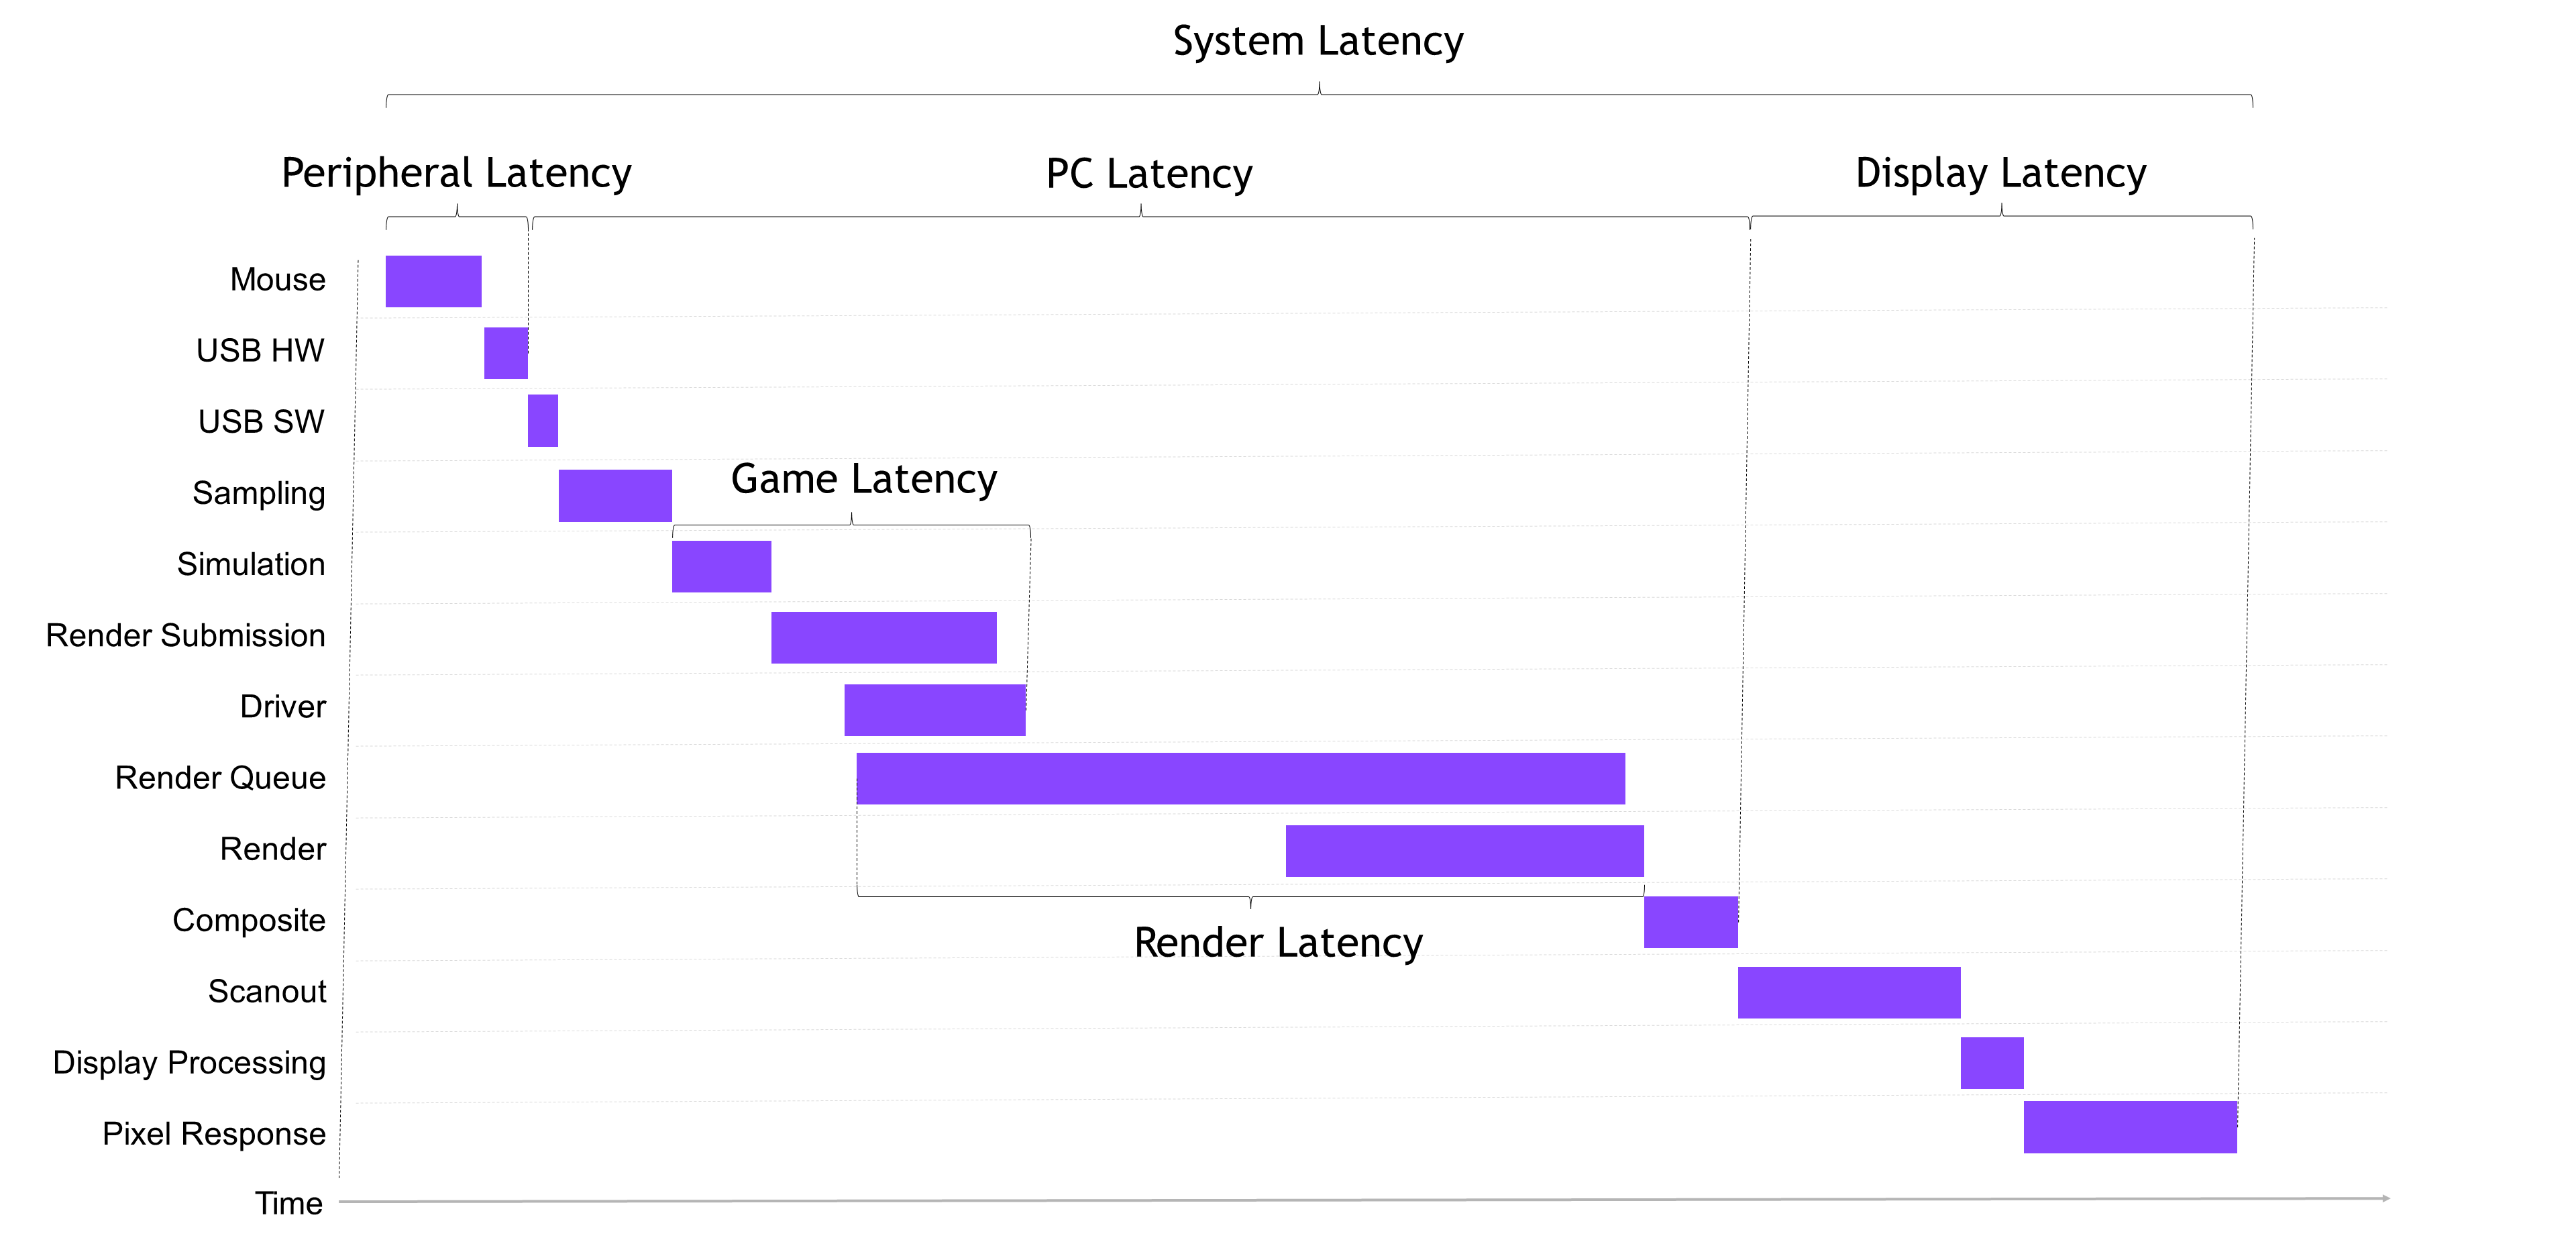
\includegraphics[width=\textwidth]{Introduzione_files/nvidia_latencypipeline.png}
	\caption{Componenti della latenza (dalla documentazione di Nvidia Reflex)}
	\label{fig:nvidia_latencypipeline}
\end{figure}

Nel momento in cui l'utente preme un pulsante sul mouse, l'azione viene registrata dal microcontroller presente all'interno del mouse stesso. Questo microcontroller è responsabile essenzialmente di tre cose:\begin{itemize}
	\item Leggere ripetutamente il sensore ottico per calcolare il movimento
	\item Ricevere le pressioni dei pulsanti sul mouse (ed eseguire il relativo \textit{debouncing})
	\item Memorizzare gli eventi in attesa che il controller USB della macchina a cui è connesso esegua il polling e riceva gli eventi tramite il protocollo USB HID (\textit{Human Interface Device})\cite{usb_hid}
\end{itemize}
La velocità con cui avviene il ciclo di lettura dei sensori del mouse è detta \textit{polling rate}, e dipende dalla qualità del mouse stesso. Valori tipici per il \textit{polling rate} sono:
\begin{itemize}
	\item \textbf{125Hz}: la velocità più comunemente usata dai mouse più economici, introduce un ritardo fino a 8ms
	\item \textbf{480Hz}: la velocità tipica dei mouse ``da gaming'' di fascia medio-bassa, introduce un ritardo fino a circa 2ms
	\item \textbf{1000Hz}: la velocità tipica dei mouse di fascia alta, introduce un ritardo fino a 1ms
	\item \textbf{Oltre 1000Hz}: raramente usato da alcuni mouse ``da gaming'' di fascia alta, tenta di ridurre il ritardo a meno di 1ms (ma si applicano considerazioni riguardo al \textit{polling rate} del sistema operativo che saranno discusse successivamente)
\end{itemize}
Quando nelle specifiche di un mouse si parla di \textit{polling rate} o di ritardo di input, il produttore si sta riferendo a questo valore e non deve essere confuso con altri fattori con lo stesso nome.

Attenzione: alcuni mouse, soprattutto quelli senza fili, riducono drasticamente il \textit{polling rate} se restano inattivi per 1-2 secondi.

Periodicamente, il sistema operativo (o il driver del controller USB) eseguono il polling dei dispositivi USB per raccogliere tutti i dati nei loro buffer. La frequenza con cui questa operazione viene eseguita è detta anch'essa \textit{polling rate}, ma non ha nulla a che vedere con il \textit{polling rate} delle specifiche del mouse.\\
Il valore esatto del \textit{polling rate} del sistema operativo dipende dall'hardware sottostante e dalla configurazione del sistema stesso (su Windows, può essere cambiato dal registro di sistema), ma il valore tipicamente usato su hardware di fascia alta è 1000Hz. Il fatto che il sistema esegua il polling a una certa velocità non rende necessariamente inutili i mouse con un \textit{polling rate} più elevato: semplicemente quando viene eseguito il polling, il sistema riceve più di un evento per volta. L'utilizzo di \textit{polling rate} elevati sul mouse è comunque utile per ridurre il \textit{jitter} del movimento (ossia irregolarità nel movimento causate dalla leggera differenza tra il \textit{polling rate} del sistema operativo e quello del mouse, che non sono in alcun modo sincronizzati) e aumentare la velocità massima del movimento che il microcontroller sul mouse stesso è in grado di rilevare prima di perdere precisione.

Attenzione: più è elevato il \textit{polling rate}, sia sul mouse che nel sistema operativo, e più aumenta il numero di eventi che il sistema e le applicazioni devono gestire, e di conseguenza l'uso di CPU. Alcune applicazioni, indipendentemente dalla potenza dell'hardware, non sono in grado di gestire quantità elevate di eventi, e in queste situazioni il ritardo introdotto dal processamento degli eventi supera di gran lunga il ritardo che si avrebbe utilizzando un \textit{polling rate} più basso ma che l'applicazione riesce a gestire correttamente.

A questo punto il sistema operativo ha ricevuto gli eventi dal controller USB e ha il compito di distribuirli alle applicazioni che li ricevono. Tipicamente questo ritardo è trascurabile, a meno di situazioni particolari come un \textit{X11 forwarding} via rete, ma questo è fuori dal contesto di questa tesi. Il metodo di recapito di queste informazioni alle applicazioni può variare in base al tipo di applicazione e di dispositivo di input, ad esempio su Windows un videogioco può ricevere eventi tramite lo stack grafico come qualsiasi altra applicazione, tramite DirectInput, o tramite XInput (per i controller per videogiochi dedicati).

Una volta ricevuti gli eventi, l'applicazione deve gestirli. Questo è uno dei principali fattori che contribuiscono al ritardo di input, e varia enormemente a seconda di come è implementata l'applicazione e dalla velocità dell'hardware sottostante. Un videogioco (o qualsiasi altra applicazione grafica interattiva) tipicamente esegue un loop di questo tipo:
\begin{itemize}
	\item Leggi gli eventi in arrivo dai dispositivi di input
	\item Esegui la logica dell'applicazione (movimento, calcoli dei danni, fisica, AI, caricamenti, eccetera)
	\item Renderizza il fotogramma su un buffer
	\item Presenta il fotogramma sul display
\end{itemize}
In ognuno di questi passaggi, ci possono essere dei ritardi che aumentano il ritardo di input:
\begin{itemize}
	\item Se gli eventi in arrivo sono processati in modo inadeguato dall'engine, potrebbero esserci dei ritardi o una notevole perdita di precisione dei movimenti (ad esempio, se legge un solo evento e scarta tutti gli altri nella coda in arrivo)
	\item Se la logica dell'applicazione richiede molto tempo di CPU per essere eseguita, o applica un qualche tipo di \textit{smoothing} sull'input, questo può introdurre diversi millisecondi di ritardo
	\item Il rendering 3D è solitamente la parte che richiede più tempo: a seconda della complessità della pipeline grafica, dal livello di dettaglio scelto, e dalla potenza dell'hardware sottostante, questo può introdurre severi ritardi: questo è il motivo principale per cui i giocatori professionisti spesso usano hardware molto potente ma giocano con il livello di dettaglio più basso possibile
	\item Il rendering può essere differito, ossia il driver video può ``fingere'' di aver eseguito i comandi che l'applicazione gli ha dato, ma in realtà li ha messi in una coda di rendering che esegue in parallelo ai fotogrammi successivi
	\item A seconda di come è implementata l'applicazione, il fotogramma renderizzato può essere visualizzato in diversi modi.\\
	La tecnica più tipicamente utilizzata è detta \textit{double-buffering}, e consiste nell'avere due buffer della dimensione dello schermo nella memoria della GPU: uno contiene il fotogramma che sta venendo trasmesso correntemente allo schermo, l'altro invece è quello su cui l'applicazione sta renderizzando il fotogramma successivo; quando il rendering è completato, si può:
	\begin{itemize}
		\item Scambiare immediatamente i due buffer e passare al prossimo fotogramma: questo fornisce la latenza migliore, ma crea ``strappi'' nell'immagine che prendono il nome di \textit{tearing}. Questa è la modalità più usata dai giocatori professionisti, ma non tutte le applicazioni sono in grado di gestire \textit{framerate} molto elevati a causa di errori di approssimazione (un esempio famoso è il videogioco del 2011 ``The Elder Scrolls V: Skyrim'', in cui la fisica è totalmente compromessa da errori di calcolo se il gioco supera i 64 FPS, cosa facilmente riproducibile su qualsiasi PC moderno)
		\item Aspettare l'intervallo di \textit{VBlank} del display, e scambiare i due buffer mentre lo schermo non sta ancora ricevendo il precedente, evitando così il \textit{tearing}: questa tecnica prende il nome di \textit{VSync} (sincronia verticale), e fornisce la qualità dell'immagine migliore a scapito però di un ritardo di input che può aumentare fino a un intero \textit{refresh} del display qualora l'applicazione manchi l'intervallo di \textit{VBlank} di poco. Associata al \textit{double-buffering}, questa tecnica limita il \textit{framerate} dell'applicazione al \textit{refresh rate} del display o ai suoi divisori (ad esempio, per un tipico display a 60Hz, l'applicazione può andare solo a 60, 30, 20, 15, ... FPS)
		\item Se il display supporta un range di \textit{refresh rate} variabile (tipicamente da 48 a 144Hz per i moderni display ``da gaming''), e il \textit{framerate} corrente ricade in quell'intervallo, può inviare immediatamente il nuovo fotogramma al driver della GPU, il quale utilizza la tecnologia VESA Adaptive Sync (o Nvidia G-Sync) per visualizzarlo senza causare \textit{tearing} e senza aumentare il ritardo di input
	\end{itemize}
	Molte applicazioni implementano inoltre, di solito come opzione, il \textit{triplo buffering}. Questa tecnica prevede l'uso di tre buffer della dimensione dello schermo nella memoria della GPU: uno è quello su cui l'applicazione renderizza il fotogramma successivo, uno è quello che l'applicazione vuole visualizzare sullo schermo, e uno è quello che è attualmente visualizzato sullo schermo. Quando il rendering di un fotogramma viene terminato, vengono scambiati i primi due buffer, quando viene raggiunto l'intervallo di \textit{VBlank} del display, vengono scambiati gli ultimi due, ma solo se è stato renderizzato almeno un fotogramma. In questo modo l'applicazione non è più legata al \textit{refresh rate} del display come con il \textit{double-buffering} tradizionale (anche se la maggior parte degli engine limitano comunque il \textit{framerate} al \textit{refresh rate} massimo del display per evitare di sprecare risorse), tuttavia introduce un intero fotogramma in più di latenza, per cui questa tecnica viene usata principalmente quando la qualità dell'immagine è più importante della latenza.
\end{itemize}

Il successivo contributore alla latenza di input è il \textit{compositor} del sistema operativo. Si possono verificare tre scenari principali:
\begin{itemize}
	\item L'applicazione bypassa completamente il \textit{compositor} utilizzando il fullscreen esclusivo e assume il controllo di uno o più display. Questa tecnica è considerata obsoleta, soprattutto perché rende difficile catturare l'output dell'applicazione o visualizzare overlay, ma è ancora usata
	\item L'applicazione chiede al sistema operativo di disattivare il \textit{compositor} mentre è in esecuzione, e crea una finestra senza bordi delle dimensioni dello schermo che vuole riempire. Questo è il caso più comune su GNU/Linux, poiché i \textit{compositor} su questa piattaforma tendono a introdurre problemi di \textit{stuttering}, ma è supportato e usato anche su Windows (da Vista in poi)
	\item L'applicazione passa regolarmente per il \textit{compositor}, creando una finestra senza bordi delle dimensioni dello schermo che vuole riempire Questa modalità introduce una latenza che dipende dal \textit{compositor} utilizzato, ma generalmente è piuttosto elevata
\end{itemize}

Il penultimo fattore che contribuisce alla latenza è il driver della GPU. I driver moderni sono infatti in grado di riconoscere un ampio set di applicazioni, e usano questa informazione per attivare o disattivare alcune funzioni, aggirare dei bug, o semplicemente per migliorare le prestazioni con ottimizzazioni specifiche per l'engine. Tra le varie funzioni che possono essere attivate, quella che introduce il maggior ritardo è la possibilità di permettere all'applicazione di prerenderizzare dei fotogrammi (tipicamente 2, ma fino a 10 nel driver di Nvidia per Windows). Dal punto di vista dell'applicazione, quei fotogrammi è come se fossero stati mandati al display, ma in realtà il driver li mette in una coda di fotogrammi che manda avanti a intervalli regolari. Questa tecnica permette di ridurre drasticamente lo \textit{stuttering} presente in molti giochi moderni causato da \textit{texture streaming}, \textit{level streaming}, \textit{garbage collection}, eccetera, migliorando così la fluidità del video, a scapito però di un elevatissimo costo in termini di latenza. Il rendering stesso dei fotogrammi può essere messo in una coda di rendering ed essere eseguito più tardi senza che l'applicazione lo sappia, riducendo il carico sull'applicazione. I driver di AMD e Nvidia offrono entrambi una modalità a bassa latenza che disattiva la prerenderizzazione dei fotogrammi, attivata di default per alcune applicazioni a latenza critica. Nvidia offre inoltre, per alcune applicazioni di cui è in grado di predire i tempi di elaborazione e rendering, la possibilità di inserire un ritardo strategico prima che gli eventi in input vengano letti; questo permette di far si che il maggior numero di eventi venga processato prima che l'applicazione si metta ad attendere il \textit{VBlank}, riducendo così la latenza di alcuni millisecondi quando il \textit{VSync} è attivo.

L'ultima causa di latenza, nonché uno dei principali contributori, è il display stesso. A differenza dei vecchi monitor CRT in cui i segnali generati dalla scheda video andavano a pilotare direttamente, tramite la connessione VGA analogica, il fascio di elettroni che disegna l'immagine, risultando in una latenza nulla, i moderni display LCD hanno un'interfaccia digitale che richiede una notevole elaborazione all'interno del display stesso.\\
Quando l'immagine arriva al display, viene memorizzata in un buffer su cui il processore all'interno del monitor può eseguire alcune elaborazioni, come lo \textit{scaling}, l'applicazione di filtri, eccetera. Sui monitor per PC tipicamente questo ha un ritardo di un fotogramma (per alcuni display anche meno, come vedremo nel capitolo sui risultati sperimentali); i televisori invece tendono a memorizzare più fotogrammi per eseguire elaborazioni più sofisticate, come l'interpolazione del movimento, aumentando notevolmente il ritardo di input, ma a volte forniscono una ``modalità gioco'' che disattiva queste funzioni, facendolo comportare come un monitor normale. Il ritardo di processamento all'interno del monitor è chiamato a volte \textit{input lag} (ritardo di input) nelle specifiche del monitor, ma è riferito al display stesso, non all'intero sistema, ed è importante non fare confusione.\\
Una volta eseguite tutte le elaborazioni necessarie, il processore nel display ha il compito di comandare il pannello LCD per visualizzare l'immagine. Il modo in cui questo avviene dipende dalla tecnologia utilizzata; il \textit{refresh} dell'intero pannello avviene solitamente dall'alto verso il basso e richiede alcuni millisecondi per essere completato (tipicamente la metà del tempo di un fotogramma); il tempo necessario affinché i pixel cambino colore è detto tempo di risposta dei pixel, ed è l'ultimo passo del percorso; tipicamente è nell'ordine di 5-10 millisecondi (nonostante i produttori spesso dichiarino tempi di 1ms o meno, questo avviene solo in condizioni particolari), ma varia molto a seconda della tecnologia utilizzata e della qualità del display stesso.

Il processo è ora terminato e l'utente può vedere l'immagine sul display; questo conclude questa sezione sui fattori chiave del ritardo di input.

\section{Funzionamento di un display}
Questa sezione introduce il funzionamento di alcuni tipi di display moderni. Non è in alcun modo esaustiva, ma è utile conoscere le basi del funzionamento prima di continuare nei capitoli successivi.

Nel corso dei decenni, sono stati sviluppati innumerevoli tipi di display, ma le tecnologie più comunemente usate oggi sono LCD TFT e OLED: i primi sono più comuni sui PC, mentre i secondi si trovano prevalentemente sugli smartphone e i televisori.\\
Una differenza fondamentale tra un display OLED e un LCD TFT, è che i primi non hanno bisogno di retroilluminazione, poiché i pixel stessi emettono luce, mentre i secondi hanno bisogno di un qualche tipo di retroilluminazione poiché si basano su filtri che bloccano o lasciano passare la luce della retroilluminazione.\\
La retroilluminazione di un display LCD può essere realizzata in diversi modi: tradizionalmente si utilizzavano dei tubi a fluorescenza (CCFL) posizionati sui lati del display che illuminano un diffusore bianco generando una retroilluminazione più o meno uniforme; i tubi CCFL sono stati poi sostituiti da dei LED bianchi, posizionati sempre sui lati ad illuminare un diffusore; più recentemente i display di fascia alta hanno iniziato ad adottare un array di LED bianchi posizionati dietro al diffusore anziché sui lati, spesso individualmente controllabili per fornire un migliore contrasto (\textit{Full Array Local Dimming}\cite{localdimming}). Alcuni display sono addirittura in grado di controllare la retroilluminazione per ogni pixel\cite{localdimming2}.\\
Con l'introduzione dei LED nella retroilluminazione, ci si scontra con il problema del dimming dei LED stessi: per simulare livelli bassi di luminosità, molti display, soprattutto quelli più economici, usano la tecnica della PWM (\textit{Pulse Width Modulation}\cite{pwm_backlight}) per accendere e spegnere molto velocemente i LED creando l'illusione all'occhio umano di valori intermedi di luminosità. La frequenza più comune per la PWM è 240Hz, ma non è l'unica. Display di fascia più alta invece sono in grado di controllare il livello di luminosità dei LED in tensione o in corrente grazie a della circuiteria più sofisticata ma più costosa.

Davanti alla retroilluminazione, nei display LCD TFT, è presente una struttura che ha il compito di far passare o bloccare la luce alterando lo stato di uno strato di cristalli liquidi. Esistono principalmente tre tecnologie per fare questo, ognuna con i suoi vantaggi e svantaggi:
\begin{itemize}
	\item TN (\textit{Twisted Nematic}): due filtri polarizzati di vetro sono posizionati rispettivamente dietro e davanti ad uno strato di cristalli liquidi, con una rotazione di 90°. Applicando una tensione allo strato di cristalli liquidi, si riesce ad alterarne la struttura in modo da variare la polarizzazione della luce che vi passa attraverso. A seconda della tensione applicata, passerà più o meno luce. Questo tipo di tecnologia è ancora oggi ampiamente utilizzata, soprattutto dai giocatori, per i bassi tempi di risposta, ma fornisce le peggiori prestazioni in termini di angolo di visione e qualità dell'immagine\cite{tftcentral_paneltech}
	\item IPS (\textit{In-Plane Switching}): a differenza dei display TN, i due filtri polarizzati sono paralleli e non ruotati di 90°. Per ottenere la rotazione di 90° del cristallo liquido, le parti interne del vetro dei due filtri sono trattate per allineare le molecole esterne del cristallo liquido alla giusta angolazione. Applicando una tensione con due elettrodi posizionati entrambi sullo stesso piano, si fa scorrere una corrente nel cristallo liquido essenzialmente parallela al piano, e si crea la rotazione che blocca o fa passare la luce. Questo è il tipo di tecnologia più utilizzata al momento, e fornisce la miglior qualità dell'immagine e angoli di visione, a scapito però di tempi di risposta relativamente alti, un maggior consumo di energia, costi più elevati, un nero poco profondo, e spesso una scarsa uniformità della retroilluminazione (detta \textit{backlight bleeding})\cite{tftcentral_paneltech}
	\item VA (\textit{Vertical Alignment}): simile a TN, ma i cristalli liquidi si allineano naturalmente in modo verticale ai filtri, bloccando il passaggio della luce. Applicando una tensione al cristallo liquido, questo si ruota verticalmente, permettendo a più o meno luce di passare in base alla tensione. Questa tecnologia è meno comune rispetto a IPS e TN, fornisce il miglior contrasto tra le tre, buoni tempi di risposta, e una qualità dell'immagine molto buona, seppur non ai livelli di un IPS; sfortunatamente è anche quella con l'angolo di visione più stretto\cite{mva1}\cite{tftcentral_paneltech}, così stretto che una sorta di effetto tunnel sui bordi è pienamente visibile anche alla distanza e angolazione di utilizzo normale, motivo per cui è poco utilizzata
\end{itemize}

Dopo aver attraversato il cristallo liquido, la luce viene colorata da uno strato di filtri colorati detto maschera (\textit{mask}) che contiene la matrice RGB che compone i pixel dello schermo.

Per controllare l'applicazione di tensione al cristallo liquido, delle linee di controllo verticale e orizzontale sono posizionate a matrice tra i pixel e permettono di controllare un TFT (\textit{Thin Film Transistor}) presente in ogni \textit{subpixel}. Questi piccolissimi transistor sono utilizzati per applicare la tensione al cristallo liquido\cite{lcdevolution}.\\
I \textit{subpixel} non sono indirizzabili individualmente (sarebbero necessarie troppe connessioni), il loro stato viene tipicamente aggiornato una linea per volta, ed è compito della matrice mantenere questo stato fino al \textit{refresh} successivo usando un condensatore assieme al transistor per mantenere l'informazione mentre le altre linee vengono aggiornate. Questa tecnica prende il nome di \textit{active matrix}\cite{lcdevolution} (matrice attiva), e tutti i display TFT moderni usano questo tipo di matrice.

Alcuni display, soprattutto quelli più economici, non utilizzano tutta l'informazione presente nell'immagine in arrivo dalla scheda video per controllare i \textit{subpixel} (ad esempio, su 8 bit per canale potrebbero usarne solo 6), così da avere una circuiteria più semplice e meno costosa, e compensano facendo uso di tecniche di \textit{dithering} spaziale e/o temporale.

\begin{figure}[h]
	\centering
	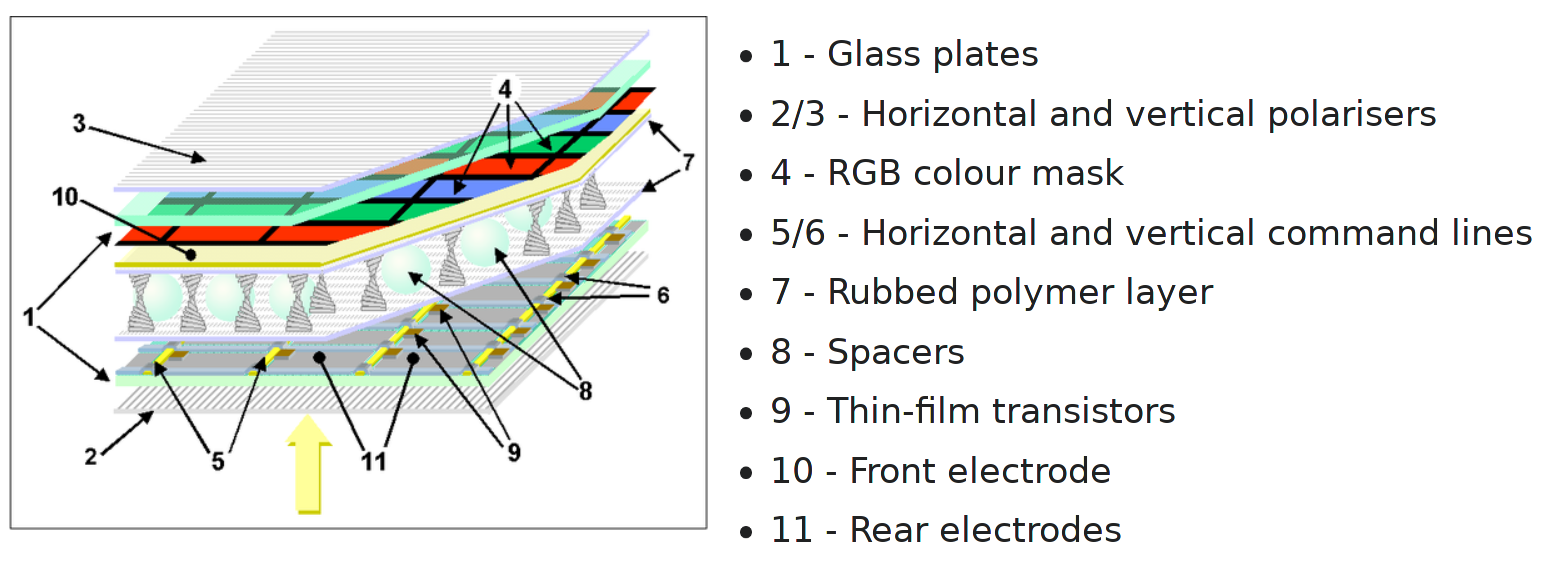
\includegraphics[width=\textwidth]{Introduzione_files/lcdtft.png}
	\caption{Struttura di un display LCD TFT (da Wikipedia, l'enciclopedia libera)}
	\label{fig:lcdtft}
\end{figure}

Per quanto riguarda i display OLED, le cose sono un po' più semplici: si tratta sostanzialmente di una matrice di piccolissimi LED organici controllati da una matrice attiva\cite{amoled1}. Ogni LED è composto da due elettrodi, uno dei quali è trasparente, e nel mezzo è presente un polimero organico che emette luce quando viene applicata una tensione. Non richiedono retroilluminazione poiché i LED emettono luce propria anziché filtrarla, il che permette di creare display trasparenti con una buona visibilità, display flessibili\cite{flexibleoleds}, e display estremamente sottili (ragione per cui sono comuni sugli smartphone). Il contrasto è eccezionale e i tempi di risposta sono buoni, tuttavia si usurano molto più velocemente rispetto ai display LCD TFT, anche se inutilizzati, l'usura non è uniforme nè nello spazio nè nei colori, soffrono di \textit{burn-in} (ossia immagini statiche come loghi visualizzate a lungo restano impresse permanentemente sul display), e il polimero organico è estremamente vulnerabile ai liquidi e all'umidità.

\begin{figure}[h]
	\centering
	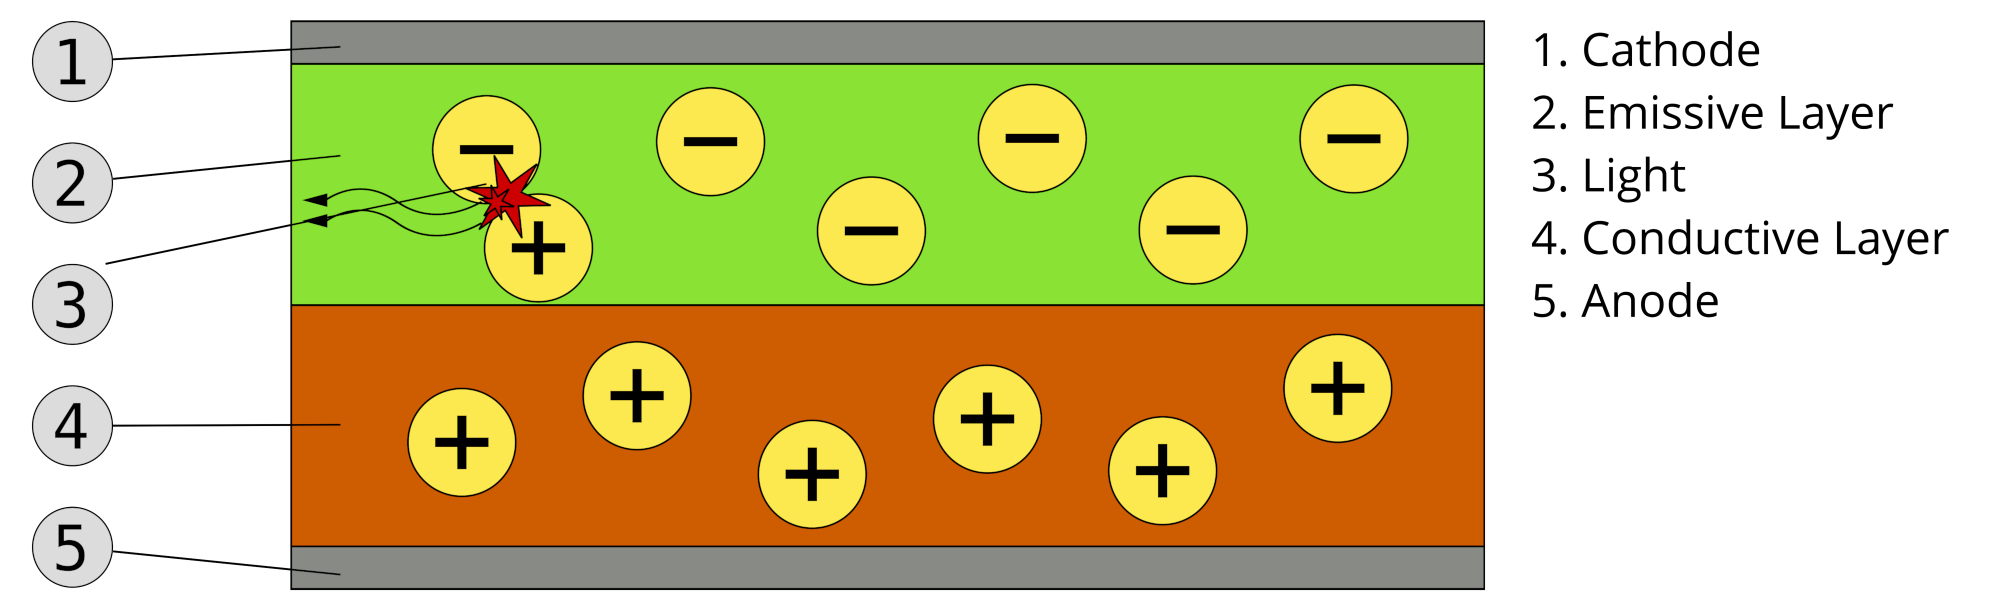
\includegraphics[width=\textwidth]{Introduzione_files/oled.png}
	\caption{Struttura di un \textit{subpixel} OLED (da Wikipedia, l'enciclopedia libera)}
	\label{fig:oled}
\end{figure}

Il passo finale nella produzione del display è uno strato protettivo di vetro per proteggere il tutto. Questo vetro può essere lucido per esaltare i colori, oppure avere una grana molto fine, per ridurre i riflessi.

Questo conclude la panoramica sulle tecnologie di display più comunemente utilizzate.

\section{Il progetto OpenLDAT}
\subsection{Storia del progetto}
L'idea del progetto OpenLDAT nasce intorno a Marzo 2019, quando durante una presentazione di Google Stadia, discutendo i problemi di latenza dell'idea di eseguire videogiochi in streaming, viene mostrata al pubblico la tabella in figura \ref{fig:stadialies}.
\begin{figure}[h]
	\centering
	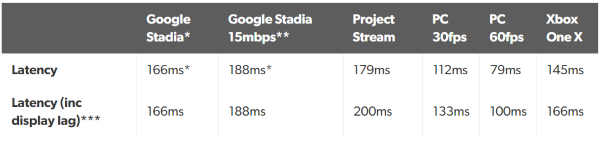
\includegraphics[width=\textwidth]{Introduzione_files/lies.png}
	\caption{Latenze secondo Google}
	\label{fig:stadialies}
\end{figure}

Ignorando per un momento il fatto che, secondo Google, Stadia ha lo stesso ritardo di input indipendentemente dal display utilizzato, che è impossibile, i numeri mostrati attirano subito l'attenzione di qualsiasi giocatore esperto, soprattutto su PC, poiché sembrano alquanto elevati. Sebbene sia vero che alcuni giochi, soprattutto quelli basati sulla storia che non richiedono di eseguire azioni rapide, hanno un ritardo elevato per migliorare la consistenza dei tempi dei fotogrammi, non è sicuramente rappresentativo nè del caso medio, nè del caso in cui la latenza è critica, come nei giochi musicali.

Vedendo questi dati, è stato deciso di costruire un semplice dispositivo per verificarli. Il dispositivo creato utilizzava un microcontroller per simulare la pressione di un tasto, la quale veniva ricevuta da un'applicazione OpenGL che generava un flash sullo schermo, che veniva rilevato da un fotoresistore collegato al microcontroller, il quale poi inviava via seriale il tempo trascorso tra l'invio del segnale e la ricezione del flash. La procedura veniva ripetuta 10 volte per avere un valore medio più accurato.

Eseguendo il test era stato ottenuto un ritardo medio di circa 50ms\cite{fdossena1}, su un display non ``da gaming''. Questo è rappresentativo del ritardo che subirebbe un videogioco programmato per avere una buona latenza sulla configurazione su cui era stato testato. Successivi test con un display a bassa latenza hanno abbassato la misura a circa 20ms.

Questa prima versione del progetto non è mai stata rilasciata per via di alcune limitazioni:
\begin{itemize}
	\item Il sensore utilizzato (un semplice fotoresistore) è relativamente lento\cite{adafruit_photores}, con un tempo di risposta di diversi millisecondi sia in salita che in discesa, il che significa che, senza un'accurata calibrazione, i risultati potrebbero essere seriamente sovrastimati
	\item Non c'era modo di regolare la soglia di attivazione del sensore se non variando delle resistenze (il sensore generava un interrupt)
	\item Il software non era in grado di gestire alcun tipo di disturbo nel segnale in arrivo dal sensore, il che causava risultati totalmente errati se veniva usato su display con retroilluminazione PWM, o dei vecchi CRT
	\item Il test funzionava solo in presenza dei flash sullo schermo, quindi non era possibile testare le diverse latenze di diverse applicazioni con questo metodo
\end{itemize}

A Novembre 2019, il lancio di Google Stadia ha attirato l'attenzione dei giornalisti del settore, i quali hanno cercato di eseguire un esperimento simile\cite{gamersnexus_stadia} \cite{gamersnexus_stadia2}, utilizzando un mouse modificato per accendere un LED quando viene premuto un tasto, e una telecamera ad alta velocità per misurare (con una risoluzione di qualche millisecondo) il tempo trascorso tra l'accensione del LED e l'inizio dell'azione sul display. L'utilizzo di metodi così ``crudi'' e manuali, anche da parte della stampa più tecnica e professionista evidenzia l'assenza di dispositivi per una facile analisi delle metriche di latenza dei display. Circa 2 anni dopo il lancio di Stadia, Google ha effettivamente raggiunto alcuni dei numeri promessi nella presentazione di Marzo 2019, ma al lancio l'opinione generale è stata pessima.

A Settembre 2020, Nvidia ha inviato un prototipo di un dispositivo chiamato Nvidia LDAT (\textit{Latency Display Analysis Tool}) a diversi giornalisti del settore\cite{gamersnexus_nvidialdat}, un dispositivo quasi del tutto analogo a quello descritto in precedenza, ma con un sensore e un software migliori. Vedere questo progetto in azione ha fornito lo stimolo a far ripartire il progetto, che è poi stato realizzato nei mesi successivi. Sfortunatamente Nvidia ha deciso di non commercializzare il dispositivo, per cui si conosce poco dei dettagli sul funzionamento, ma verrà comunque discusso nel capitolo successivo sullo stato dell'arte.

Nel periodo tra Dicembre 2020 e Marzo 2021 è stato svolto gran parte del lavoro sul progetto OpenLDAT che, assieme ai dati sperimentali, è oggetto di questa tesi.

Nel periodo tra Marzo 2021 e Giugno 2021 è stata scritta questa tesi, sono stati eseguiti test su vari tipi di display, e sono state fatte migliorie agli algoritmi per assicurarne il buon funzionamento sul maggior numero possibile di display.

\subsection{Obiettivi del progetto}
Il progetto OpenLDAT si pone i seguenti obiettivi principali:
\begin{itemize}
	\item Fornire agli utenti un dispositivo per poter misurare, sia automaticamente che interattivamente, la latenza totale del proprio sistema, nel modo più accurato possibile, e permettendo il confronto tra sistemi e scenari diversi
	\item Rendere il dispositivo utilizzabile sul maggior numero possibile di display, anche in presenza forti disturbi come una retroilluminazione PWM
	\item Utilizzare il sensore nel dispositivo per fornire ulteriori metriche che non riguardano esclusivamente la latenza, ma anche la qualità del display, come una stima dei tempi di risposta reali dei pixel in diversi scenari
	\item Rendere il dispositivo facilmente costruibile, utilizzando componenti \textit{off-the-shelf}, facilmente reperibili, dai costi contenuti, e un software che non richieda calibrazioni
	\item Distribuire tutte le schematiche del dispositivo e il software su licenza libera, per consentire agli utenti di capirne il funzionamento e potenzialmente anche di apportare migliorie
\end{itemize}

Inizialmente, il progetto è rivolto principalmente a un pubblico tecnico, poiché è necessario sapersi assemblare il dispositivo da sè; qualora ci fosse interesse sufficiente per il progetto, però, diventerebbe possibile distribuirlo come prodotto finito e pronto all'uso; in questo caso il target si espanderebbe notevolmente, e diventerebbe usufruibile anche a un pubblico di giornalisti di tecnologia se non addirittura potenziali acquirenti in cerca di un nuovo monitor.

\subsection{Struttura del repository del progetto}
Tutti i file relativi al progetto OpenLDAT sono disponibili sul relativo repository GitHub\footnote{\url{https://github.com/adolfintel/OpenLDAT}}. %è privato fino a fine tesi

Il respository è strutturato in questo modo:\begin{itemize}
	\item \texttt{App}: contiene il codice dell'applicazione OpenLDAT per PC e i file necessari per creare i \textit{package} distribuibili. \begin{itemize}
		\item \texttt{OpenLDAT}: progetto dell'applicazione per NetBeans
		\item \texttt{Packaging stuff}: file necessari per creare i \textit{package} distribuibili per Windows, GNU/Linux e MacOS
	\end{itemize}
	\item \texttt{Device}: contiene tutti i file relativi al dispositivo fisico OpenLDAT: \begin{itemize}
		\item \texttt{Case}: modelli 3D per il case stampabile e relative istruzioni
		\item \texttt{Firmware}: file relativi al firmware del dispositivo \begin{itemize}
			\item \texttt{OpenLDAT}: progetto del firmware per Arduino IDE
			\item \texttt{boards.txt}: dichiarazione del dispositivo per Arduino IDE
			\item \texttt{Libraries.zip}: copia di backup delle librerie necessarie per compilare il firmware, qualora non fossero più disponibili in futuro
			\item \texttt{Prebuilt}: firmware precompilato per programmare il dispositivo senza Arduino IDE
		\end{itemize}
		\item \texttt{Hardware}: file relativi al circuito del dispositivo: \begin{itemize}
			\item \texttt{OpenLDAT\_Model1.fzz}: progetto del dispositivo per Fritzing
			\item \texttt{gerber}: file del PCB del dispositivo in formato standard gerber per la stampa
		\end{itemize}
	\end{itemize}
	\item \texttt{Docs}: documentazione del dispositivo e dell'applicazione, in inglese
\end{itemize}

Questo conclude il capitolo introduttivo. Nei capitoli successivi verrà discusso lo stato dell'arte, confrontando OpenLDAT con progetti, dopodiché verrà introdotto il dispositivo stesso.

